% !TEX root = mfe.tex


\newcommand{\base}[1]{\ensuremath{\mathrm{#1}}\xspace}
\newcommand{\baseA}{\base{A}}
\newcommand{\baseT}{\base{T}}
\newcommand{\baseG}{\base{G}}
\newcommand{\baseC}{\base{C}}
\newcommand{\baseU}{\base{U}}

\section{Introduction}

The  {\em primary structure} of a DNA strand is simply a word   over the alphabet  $\{\baseA, \baseC, \baseG, \baseT\}$, or  $\{\baseA, \baseC, \baseG, \baseU\}$ for RNA.  
Bases may bond in pairs, \baseA binds to \baseT and \baseC binds to \baseG, and a set of such pairings for a strand is called a {\em secondary structure} as shown in {\cref{fig:sec struct}(a)}; typically each strand has exponentially many possible secondary structures.\footnote{A secondary structure, along with a set of experimental conditions,  induces one or more 3D structures called tertiary structures---a complication we will not be concerned with in this paper since, unlike proteins, it is fortunate that DNA/RNA interactions are sufficiently chemically simple that that somewhat elementary secondary structure model is sufficient for useful structural prediction.} 
Mainly, what practitioners care about are probabilities of a given secondary structure or class of secondary structures. 
For that, each secondary structure~$s$ has an associated, typically negative, real valued {\em free energy} $\Delta G(s)$, where more negative is deemed more favourable.  
Thus the most favourable is the secondary structure, or structures, with minimum free energy (MFE). 
More generally, the Boltzman distribution is  a probability distribution on secondary structures $s$ at chemical equilibrium:  
the probability of~$s$ is  $p(s) = \frac{1}{Z} \mathrm{e}^{- \Delta G(s)/k_\mathrm{B}T}  $ where $Z$ is a normalisation factor called the partition function: 
\begin{equation}\label{eq:pf}
	Z  = \sum_{s\in\Omega} \mathrm{e}^{- \Delta G(s)/k_\mathrm{B}T} 
\end{equation}
that is, an exponentially weighted sum of the free energies over the set~$\Omega$ of all secondary structures, 
where~$k_\mathrm{B}$ is Boltzmann's constant and $T$ is temperature in Kelvin. 

\begin{table}[t]
	\centering
	\begin{tabular}{ p{5cm}||p{5cm}|p{5cm}  }
		%\hline
		
		Input type& MFE & Partition function\\ 
		
		\hline\hline
		
		Single strand   &   $\mathcal{O}(N^4)$ \ \   \cite{zukeroptimal,zukerrna, nussinov1978algorithms, nussinov1980fast,waterman1986rapid}  &   $\mathcal{O}(N^4)$ \ \  \cite{mccaskill1990equilibrium}     \\  \hline
		Multiple strands, bounded,\newline i.e.~$c= \mathcal{O}(1)$ strands &  $\mathcal{O}(N^4 (c-1)!)$ \ \  {\bf [Theorem~\ref{thm:main}]}   &   $\mathcal{O}(N^4 (c-1)!)$  \ \ \  \cite{dirks2007thermodynamic}\footref{ft:N3}    \\ \hline
		Multiple strands, unbounded,\newline i.e.~$\mathcal{O}(N)$ strands &  APX-hard \ \   \cite{condon2021predicting}  &  Open problem   \\ \hline
	\end{tabular}\vspace{-1.5ex}
	\caption{\label{table}\small
		Some algorithmic results for MFE and partition function for unpseudoknoted\footref{ft:pseudoknot} nucleic acid systems.
		$N$ is the total number of bases of all strand(s) in the system (i.e.~sum of strand lengths).
		Results are shown for input being a single strand, 
		multiple strands bounded by a constant or unbounded/growing with~$N$. 
		Note that in the literature the polynomial is sometimes written to the power 3 (e.g.~$\mathcal{O}(N^3 ...)$), but this is for a restricted ``relaxation'' of the model.\footref{ft:N3}  
	}
\end{table}

Decades ago, the deep relationship between secondary structures and dynamic programming algorithms was established~\cite{zukeroptimal,zukerrna, nussinov1978algorithms, nussinov1980fast,waterman1986rapid, mccaskill1990equilibrium}.  
If a secondary structure can be drawn as a polymer graph  without edge crossings it is called unpseudoknotted  (\cref{fig:sec struct}(c)).
The earliest polynomial time algorithms were for single-stranded  unpseudoknotted secondary structures, with the absence of crossings allowing for planar decompositions of secondary structures that are suited  to dynamic programming techniques.\footnote{Exclusion of pseudoknots is usually founded on both modelling and algorithmic considerations. Energy models for pseudoknots are difficult to formulate due to the increased significance of geometric issues and tertiary interactions \cite{dirks2007thermodynamic}. If pseudoknots are permitted, it is known that the MFE prediction is NP-hard even for a single strand \cite{akutsu2000dynamic,lyngso2000pseudoknots,lyngso2000rna}.The first NP-hardness results \cite{akutsu2000dynamic,lyngso2000pseudoknots} used a simple energy model called the stacking model where only consecutive base pairs forming a stack contribute to the free energy of a secondary structure. These hardness results with relatively simple energy models, make it seems unlikely that the MFE prediction problem will be easier in the case of more complicated energy models~\cite{condon2021predicting}. But, dynamic programming algorithms are still possible for restricted classes of pseudoknots, for both MFE prediction \cite{rivas1999dynamic, uemura1999tree, chen2009n, jabbari2018knotty, reeder2004design} and partition function \cite{dirks2003partition, dirks2004algorithm}. \label{ft:pseudoknot}}  
For a single RNA/DNA strand, both MFE and partition function are computable in $\mathcal{O}(N^4)$ time (\cref{table}),  using the standard  energy model\footnote{This model is variably called the nearest neighbour model, the Turner model, and loop energy model. 
Versions of the model have been implemented in software suites such as NUPACK~\cite{dirks2007thermodynamic,dirks2004algorithm,fornace2020unified}, ViennaRNA~\cite{viennaRNA} and mfold~\cite{mfold}, for both RNA and DNA~\cite{santalucia1998unified,santa}.} that will be formally defined in \cref{sec:mfe}. 

Work in DNA computing~\cite{algoSST,squareRoot,cargoSorting,SIMDDNA,celltimer2017fernshulman,Chatterjee2017,seelig2006enzyme,zhang2011dynamic}, and nucleic acid nanotechnology more generally~\cite{geary2014single,woo2011programmable}, involves building molecular systems and structures with, to date, hundreds, and soon, thousands, of interacting strands, so there is a need for better algorithms for these multi-stranded `inverse design problems'~\cite{churkin2018design,nuad}.  
And, of course, biologists need to understand molecular structure in order to understand and predict molecular interactions. 
However, when there are multiple interacting strands, the situation becomes significantly more complicated than the single-stranded case for two reasons:  
First, for a secondary structure to be unpseudoknotted, it implies there should be {\em at least one} permutation of the strands without crossings on the polymer graph~\cite{dirks2007thermodynamic} (\cref{fig:sec struct}). 
Second, if strand types are repeated then 
so-called {\em rotational symmetries} (\cref{fig:sym}) arise that need to be accounted for in the model to match the underlying statistical mechanics\footnote{This fact from statistical mechanics is discussed in some papers~\cite{dirks2007thermodynamic,hofacker2012symmetric}, although we've not found its full derivation in the modern nucleic-acid algorithmic literature. We leave a first-principles derivation for future work.\label{ft:statmech}}, otherwise structures may be over- or undercounted, leading to incorrect probabilities in the Boltzmann distribution, in other words: incorrect predicted free energy of a secondary structure.

% A future version of this paper will include a

For multiple strands, albeit a constant number $c = \mathcal{O}(1)$, 
Dirks,  Bois, Schaeffer, Winfree and  
Pierce~\cite{dirks2007thermodynamic} gave a polynomial time partition function algorithm running in time $\mathcal{O}(N^4 (c-1)!)$.\footnote{We note that Dirks et al~\cite{dirks2007thermodynamic}, and others in field~\cite{zukeroptimal,zukerrna,condon2021predicting,waterman1986rapid,mccaskill1990equilibrium,boehmer2024rna}, often state the run time with 3  instead of 4 in the exponent (i.e. $\mathcal{O}(N^3)$ for single stranded and $\mathcal{O}(N^3 (c-1)!)$ for multistranded). This reduction comes from changing the standard energy model by putting some restrictions on the size of interior loops (\cref{fig:sec struct}), or by enforcing certain mild conditions on the energy parameters for the interior loops  \cite{lyngso1999fast,hofacker2012symmetric}, we do not assume these additional assumptions in this work.\label{ft:N3} Note that our time/space complexity could benefit from such model changes for example, via reduction of the upper bound in \cref{lem:polyub}}. 
The first problem goes away by simply assuming $c$ is a constant;
but if the number of strands is non-constant, in particular $c = \mathcal{O}(N)$, 
Codon, Hajiaghayi and Thachuk~\cite{condon2021predicting} showed MFE is NP-hard, and even APX-hard.\footnote{This hardness result holds whether or not rotational symmetries are accounted for in the energy model.} 
For the second, rotational symmetry, problem, in order to compute partition function, Dirks et al~\cite{dirks2007thermodynamic} found an algebraic link between the overcounting and the rotational symmetry correction problems, which allowed both to be solved simultaneously, aided by the exponential nature of the partition function.  
Surprisingly, that trick does not work for MFE:
Since MFE prediction is minimization-based, 
there is no secondary structure overcounting problem in MFE prediction---repeated secondary structures will not change the outcome of minimization, unlike the partition function which is summation-based.
Hence, the absence of the overcounting problem makes MFE prediction harder to solve, and was left open by Dirks et al~\cite{dirks2007thermodynamic}.
For the special case of two strands, Hofacker, Reidys, and Stadler~\cite{hofacker2012symmetric} gave an $\mathcal{O}(N^6)$  algorithm. In this paper, we propose an efficient solution to the $\mathcal{O}(1)$ strand MFE problem, the first that runs in polynomial time. 



\subsection{Statement of main result}
Our main result is the following theorem, whose proof is in \cref{sec:analysis}: 

\begin{restatable}{theorem}{main} 
	\label{thm:main}
	There is an $\mathcal{O}(N^4(c-1)!)$ time and $\mathcal{O}(N^4)$ space algorithm for the 
	Minimum Free Energy unpseudoknotted secondary structure prediction problem, including rotational symmetry, 
	for a set of $c = \mathcal{O}(1)$ DNA or RNA strands of  total length  $N$ bases. 
\end{restatable}

In \cref{sec:analysis} we give a time-space trade-off for our result, by showing a variation of the algorithm runs in $\mathcal{O}(N^4 \log N (c-1)!)$ time but $\mathcal{O}(N^3)$ space.  


We use the standard~\cite{dirks2007thermodynamic} definition of free energy (\cref{eq:DGss}) of multistranded unpseudoknotted secondary structures, which includes rotational symmetry, see \cref{sec:mfe} for formal definitions.  
We first give an extensive overview of the proof and paper structure, followed by future work. 


\begin{figure}[t]
	\centering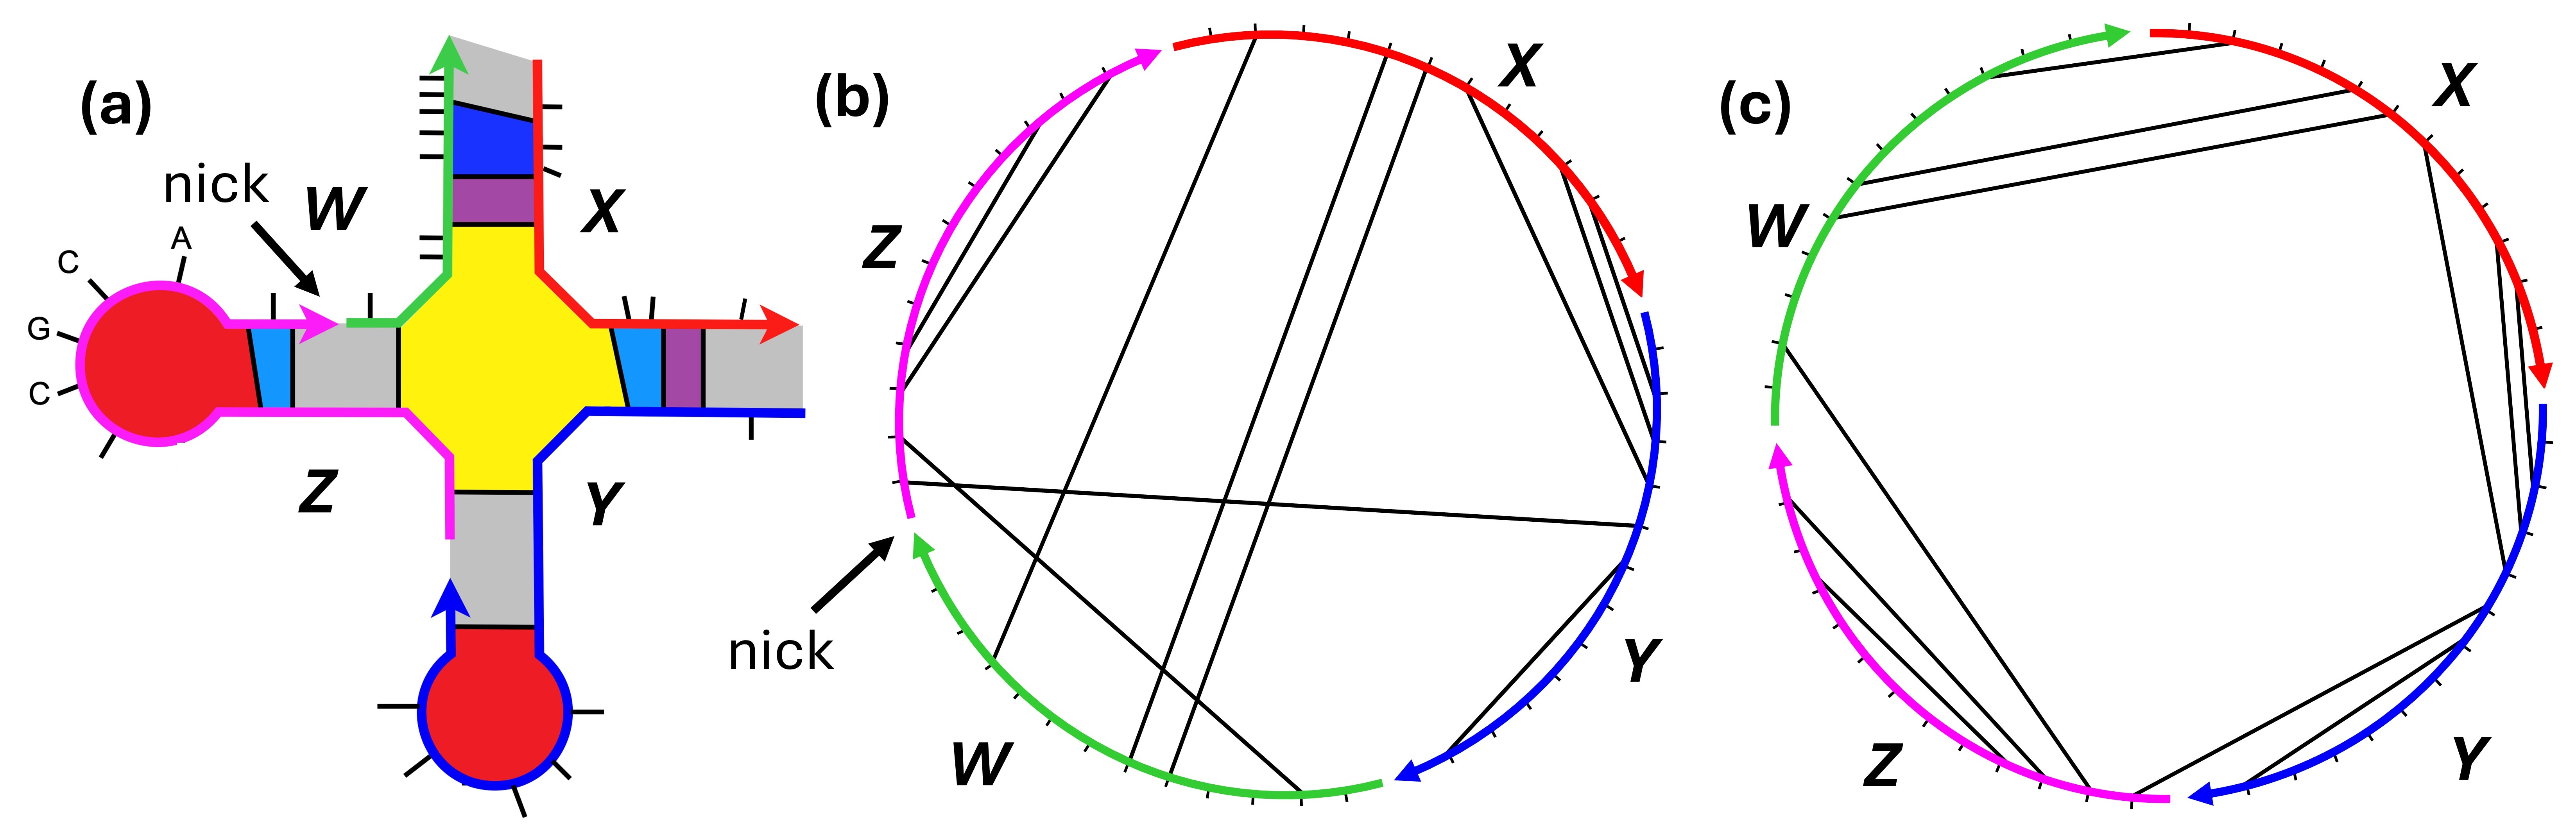
\includegraphics[width=0.9\textwidth]{figures/ss.jpg}
	\caption{
		A  DNA (or RNA) secondary structure $S$ with $c=4$ strands and two of its $(c-1)!=6$ polymer graphs. 
		(a) One of the many possible secondary structures for four DNA strands $W,X,Y,Z$. 
		Short black lines represent DNA bases (a few are shown $\ldots \baseC, \baseG, \baseC, \baseA \ldots$), and long lines represent base pairs (drawing not to scale). 
		Loops are colour-coded as follows:  stack=purple, multiloop=yellow, hairpin=red, bulge=light blue, internal=dark blue, external=grey.    
		Black arrow: the small gap between two strands is called a {\em nick}. 
		(b)~Polymer graph for the strand ordering $\pi' = WZXY$, denoted \PolySpiPrime, showing base-pair crossings.
		(c)~By  reordering to $\pi = WXYZ$ we get another polymer graph \PolySpi for $S$, without crossings, hence  $S$ is unpseudoknotted. 
	}
	\label{fig:sec struct}
	
\end{figure}

\subsection{Proof overview and paper structure}\label{sec:intuition}

\subsubsection{The main challenge: handling rotational symmetry}

Typically, each DNA base pair that forms represent a decrease (improvement in favourability) in free energy---although not always. 
In a multi-stranded system, when several strands bind together the entropy of the overall system is decreased since there are now less states due to their being less free molecules.  
Thus the energy model for multistranded systems includes an entropic {\em association penalty} (typically positive) for every extra strand, beyond the first, bound into a multistranded molecular  complex~\cite{dirks2007thermodynamic}. 
However, statistical mechanics tells us to be careful about symmetry: with multiple identical strands in a complex it is possible that the complex is rotationally symmetric, 
intuitively  there are several complexes, identical up to rotation of their polymer graphs (\cref{fig:sym}).\footnote{Formally, we mean the permutation representing the complex is rotationally symmetric.} 
These so-called indistinguishable complexes, in turn imply that a (positive) penalty should be applied to account for the difference in entropy between a similar, but distinguishable, complex without  rotational symmetry~\cite{bormashenko2019entropy,atkins2023atkins,silbey2022physical,fornace2020unified}.\footref{ft:statmech} 
\cref{sec:mfe} gives definitions needed  to formalise these concepts, including: DNA,  
unpseudoknotted secondary structure, polymer graph,  
free energy including rotational symmetry (\cref{eq:DGss}) and MFE (\cref{eq:MFE}). In particular, \cref{sec:sym} gives a  group-theoretic definition of rotational symmetry, to help formalise some of the prior work.

\subsubsection{General approach to find the true MFE}
One obvious idea might be to find a dynamic programming algorithm that directly handles rotational symmetry. 
However, this approache suffers from rotational symmetry being a {\em global property} of an entire system state (secondary structure), whereas dynamic programming relies on piecing together subproblems that are individually unaware of the global context---or more precisely, may be used in multiple global contexts whether symmetric or not.  

Instead, our strategy is to first compute what we call the {\em \symnMFE} (\snMFE) that (incorrectly) assumes all strands are distinct and thus does not compute correct free energies for rotational symmetries. 
We use  Dirks et al's \snMFE algorithm~\cite{dirks2007thermodynamic},  that assumes all strands are distinct, but  augmented to return extra dynamic programming matrices (\cref{algo:1} in \cref{sec:AlgoMFE}). 
We use these extra matrices to compute the required symmetry correction to that \snMFE value using a backtracking algorithm, as  follows.



\subsubsection{Polynomial upper bound: intuition for \cref{sec:ub}} 
Our goal is to show that, after running our augmentation of the known algorithm for \snMFE, we have implicit access to a collection of secondary structures that are `not too far' from the true MFE---where by `not too far' we mean we have a polynomial bound on the number of structures to be  considered by another fast (``backtracking'') algorithm that finds the true MFE structure.


First, 
to see how we find this polynomial bound,  imagine  the augmented
\snMFE algorithm finds that the secondary structure with \snMFE is  rotationally {\em  asymmetric}, hence we are done, we know that the \snMFE value is in fact the true MFE. 
Otherwise, we have a {\em rotationally symmetric} secondary structure: ideally we would like to compute it's rotational symmetry degree $R$ (takes linear time in the size of the secondary structure) and then return  $\mathrm{\snMFE} + k_\mathrm{B} T \log R$ as the true MFE, but this approach is doomed to fail since there could also be structures with lower true MFE, i.e.~in the real interval $[\mathrm{\snMFE}, \ \mathrm{\snMFE} + k_\mathrm{B} T \log R) \subset \mathbb{R}$. 



Leveraging the two properties of being (a) unpseudoknotted and (b) rotationally symmetric, in \cref{sec:ub} we define a class of cuts of a structure's polymer graph (\cref{fig:sec struct}) that we call {\em pizza cuts}, or, more formally, \emph{admissible symmetric backbone cuts} (\cref{def:admissible}). 
These cuts are radially symmetric, hence the name pizza cut---how one slices a pizza from disk-edge to centre.
In \cref{lem:ub,lem:ub2}, we show that there are at most a polynomial number of pizza cuts that symmetric structures may have. 



Then, when we do a backtracking-based search (below), 
through the dynamic programming matrices from the structure(s) with \snMFE, to larger free energies:  
if we find two different symmetric pizzas, but with the same pizza cuts,  we make a new pizza, by swapping a slice from one with a slice from the other.  
We prove that the new pizza is (a) guaranteed to be asymmetric and (b)~has free energy sandwiched between the {\snMFE} values of  two symmetric structures  (\cref{lem:sand,lem:ub2}). 
Moreover, this new structure's free energy is the true MFE. 
Otherwise we either find a symmetric structure (we output its naive free energy as the true MFE), or we reach a contradiction (i.e.~which can not happen) by reaching the polynomial bound having exhausted the set of all \emph{admissible symmetric backbone cuts}. In all cases the true MFE and its structure are output. 




\subsubsection{Backtracking to find the true MFE: intuition for \cref{sec:BT}} 

It remains to show how we will do the backtracking search mentioned above. 
In \cref{sec:BT} we analyse the  backtracking algorithm, which is given in \cref{algo:2} in \cref{app:backalgo}, and  
is a polynomial time  algorithm over the exponentially large set of structures `close' to the true MFE value. 
It scans all secondary structures within an energy level starting with the \symnMFE (\snMFE) energy level, it goes on to sequentially scan higher levels in low-to-high order. 
The scanning process at any energy level $\mathcal{E}$  guarantees that each secondary structure that belongs to $\mathcal{E}$ should be scanned exactly once. 

The backtracking algorithm will run until one of the following conditions occurs:
(1) It scans an asymmetric secondary structure $S$, or 
(2) it exceeds the polynomial upper bound $\mathcal{U}$ of the number of symmetric secondary structures (i.e. the number of distinct  pizza cuts) to be scanned, or 
(3) the backtracking will start scanning a new energy level $\mathcal{E}' > \mathcal{B}$, where $\mathcal{B}$ is the current best candidate for MFE (the starting value for $\mathcal{B}$ is  $\mathcal{B} = \mathrm{\snMFE} + k_\mathrm{B} \log v(\pi)$ where $v(\pi)$ is the highest degree of rotational symmetry, \cref{def:sym}). 
Then, based on the condition that will occur, the algorithm directly returns the true MFE, and a secondary structure which has the true MFE will also be constructed. 
The short proof of \cref{thm:main} in \cref{sec:analysis} ties these results together to give the final analysis of our main result.


\subsection{Future work}
Our algorithm runs in polynomial time $\mathcal{O}(N^4 (c-1)!)$ for the case of $c=\mathcal{O}(1)$ strands, the $(c-1)!$ term coming from the fact that our algorithm, as well as Dirks et al~\cite{dirks2007thermodynamic}, is assumed to be called from an outer  loop that explicitly tries all $(c-1)!$ cyclic strand permutations. 
Can we increase the number of strands and still have a polynomial time algorithm? We know ``not by much'', since the problem is NP-complete when $c=\mathcal{O}(N)$~\cite{condon2021predicting}. 
Interestingly, Boehmer, Berkemer, Will, and Ponty~\cite{boehmer2024rna} recently reduced the $c$-strand parameterized running time for computing \symnMFE (i.e.~ignoring rotational symmetry) and partition function from factorial, $\mathcal{O}(N^4 (c-1)!)$, to exponential, $\mathcal{O}(N^4  3^c)$.\footref{ft:N3}  
It is feasible that our MFE algorithm could be augmented via this result.

Our MFE algorithm exploits a polynomial upper bound, $\mathcal{U}$, on the number of so-called symmetric secondary structures, or distinct  pizza cuts.  That bound is linear in ``most'' cases (\cref{lem:even}), but quadratic in one special subcase (\cref{lem:ub2}) of 2-fold rotational symmetry with a central internal loop. Reducing  that special case to linear would subtract one from  our algorithm's running time exponent.

\cref{table} shows the open problem for partition function on multiple strands. Intuitively, it seems that  partition function should be at least as hard as MFE, however that intuition is tempered by the fact that Dirks et al's approach for partition function did not carry over to MFE, hence this is an open problem. Indeed, our paper brings extra techniques to handle multi-stranded MFE.   

More generally, the computational complexity of partition function for DNA/RNA strands is less well understood than MFE. 
For example, are there settings where partition function, or problems counting numbers of structures, are {\#}P-complete? 